\chapter{Distance education}

Distance education is not only a phenomenon of the few last decades, but can be traced at least back to the 18th century, when Caleb Phillipps posted an advertisment called ``Teacher of the New Method of Short Hand'' in Boston Gazette, saying ``Persons in the Country desirous to Learn this Art, may by having the several Lessons sent weekly to them, be as perfectly instructed as those that live in Boston.'' \cite{1}

With the development of the Internet and its general accessibility in the developed world, providing distance education has become much easier and has spread widely. In some countries tuition rates are high and young people take loans. This topic is covered in a fitting way by John Oliver in his show \cite{2}. The flexibility and low cost of distatnce education over the Internet gives people, who wouldn't be otherwise able to attend a traditional university, an opportunity to gain knowledge and train skills from their homes \cite{3}.

Students in the deveopling world are also taking the advantage of educational content available on the Internet. Several of the top U.S. universities, like Harvard, Stanford or MIT, put some of their materials on so called MOOCs (Massive Open Online Course) like Coursea, edX or Udacity. This content is then available to anyone with a computer and Internet connection and knowledge of the language. A fitting example is Kepler - non profit university project in Rwanda \cite{5}. The goal of this project is to ``provide an American-accredited degree, a world class education, and a clear path to good jobs for thousands of students for around \$1,000 tuition per year.'' \cite{6}

\section{Current systems}
In the next few pragraph I will try to pick some of the current distance education systems available on the Internet for free. This list is not complete and is only meant to give the reader a notion of available technologies and their paradigms, which project into the project of Vector Screencast.

\subsection{Moodle}
Moodle \cite{7} is an open-source project providing a robust tool for creating custom learning materials and providing them to students. Anyone can download the source code of Moodle and deploy it on his own server.

This tool is used by millions of users \cite{8}.

\subsection{Coursera}
The mission of Coursera is to ``provide universal access to the world’s best education.'' \cite{9} Anyone can, for free, go through materials published by universities and other organizations aimed at education.

Courses at Coursera consist mainly of video lectures commonly with a transcript and a presentation document attached to. These videos can be viewed directly in the browser on demand or downloaded to user's computer. After studing the materials, students can submit asignments solutions and take quizes and receive a Verified Certificate for the accomplishement of the course. These certificates are not free.

Most of the courses are in English and only a few of the courses are also translated into other languages. It is not possible for everyone to publish his materials through Coursera.

\subsection{Youtube.com}
The Youtube web service \cite{10} is not primarily designed to be an educational resource. Youtube allows people to create their own video content and share it with other Internet users for free. Youtube was launched in 2005 and has became one of the most frequently visited websites on the Internet according to Alexa Internet \cite{11}. Uploading video to Youtube is free, advertisment is displayed to the user while watching videos though.

The ease of making original-created videos available and the wide audience makes Youtube a perfect place for all individuals and organizations, who want to share their ideas or any video materials. Many educational channels can be found here, for example Numberphile \cite{12}, Veritasium \cite{13}, and Khan Academy \cite{14}.

Youtube videos can be viewed only online in a web browser or a specialized application. There are only unofficial tools for downloading these videos.

The form and content of the video is not limited anyhow, as long as does not violate the terms of the service. Video can have a text description which might contain the transcription of the video content and any subtitles can be attached to a video. Youtube also downscales videos to multiple resolutions so they can be also viewed using low speed Internet connections.

\subsection{Khan Academy}
A similar service to Coursera is Khan Academy. Khan Academy originated in 2004 when it's founder, Salman Khan, began tutoring his cousin over an instant messenger via drawing diagrams with a computer mouse. Salman then started to capture these videos and put them on Youtube, so someone could watch them later.

The format of Khan Academy videos remained the same. A person draws diagrams on a computer canvas and comments the subject with his voice. These videos are then uploaded to Youtube and embeded on the Khan Academy website \cite{14}. Apart form the video lectures, the website also contains exercises and quizes to encourage students in learning. The pace of the lesson depends on the student. He can pause the videos or watch them multiple times before continuing with the lesson~\ref{fig:khan-screen}.

Most of the videos are recorded in English, but many of the videos are translated into other languages - by replacing the audio track with a different one or with subtitles.

One of the projects working on the localization of Khan Academy videos is a czech branch called Khanova Škola \cite{15}.

\begin{figure}
	\centering
	%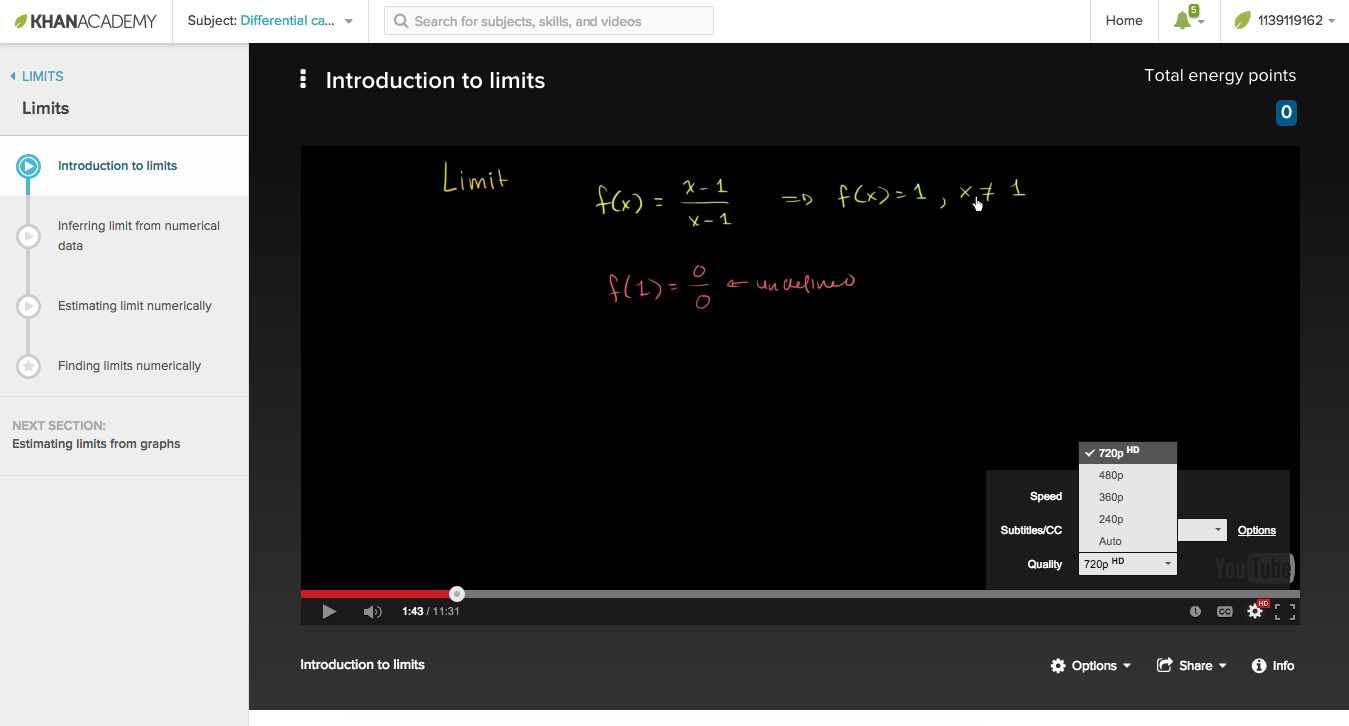
\includegraphics[width=30mm]{../img/khan-academy-screenshot.png}
	\caption{Khan Academy lesson}
	\label{fig:khan-screen}
\end{figure}